\chapter{Design and Implementation}
\label{chap:implementation}

In this chapter the design and implementation of the prototype for the Austrian parliament is described. First of all, in Section \ref{sec:architecture} the overall architecture and the different components are being discussed. The more detailed description of the implementation is divided into four sections: Section \ref{sec:data_extraction_transforming} which shows how the protocols were accessed and transformed into structured data, section \ref{sec:export_db} which discusses the database export, section \ref{sec:analysis} which describes which analysis is done over the available data and section \ref{sec:visualization} which shows how the information gets displayed.

\section{Architecture}
\label{sec:architecture}
Figure \ref{fig:general_architecture} shows the general architecture of the prototype which was implemented. The ETL-Application brings the data from the protocols in the database whereas the web server application visualizes the results and shows statistics and graphs for the given data. The ETL-Application is implemented using the ETL pattern. This means that there are three distinct steps: Extract - Transform - Load. First the application reads an RSS feed which contains all the protocols for one legislative period and the politician profiles (Extract). The retrieved HTML-files get parsed and are transformed into Java objects (Transform) which get loaded into a relational database\footnote{in the prototype, a PostgreSQL database was used} (Load). To visualize the then available data, the analysis engine queries the database, preforms analysis on it and converts the data in a form which can be displayed (e.g. a graph structure). Furthermore, this data is made available via RESTful web services. The Polymer web application accesses these web services and shows graphs and statistics. All the components will be described in more detailed in the later sections.

\begin{figure}
	\centering
	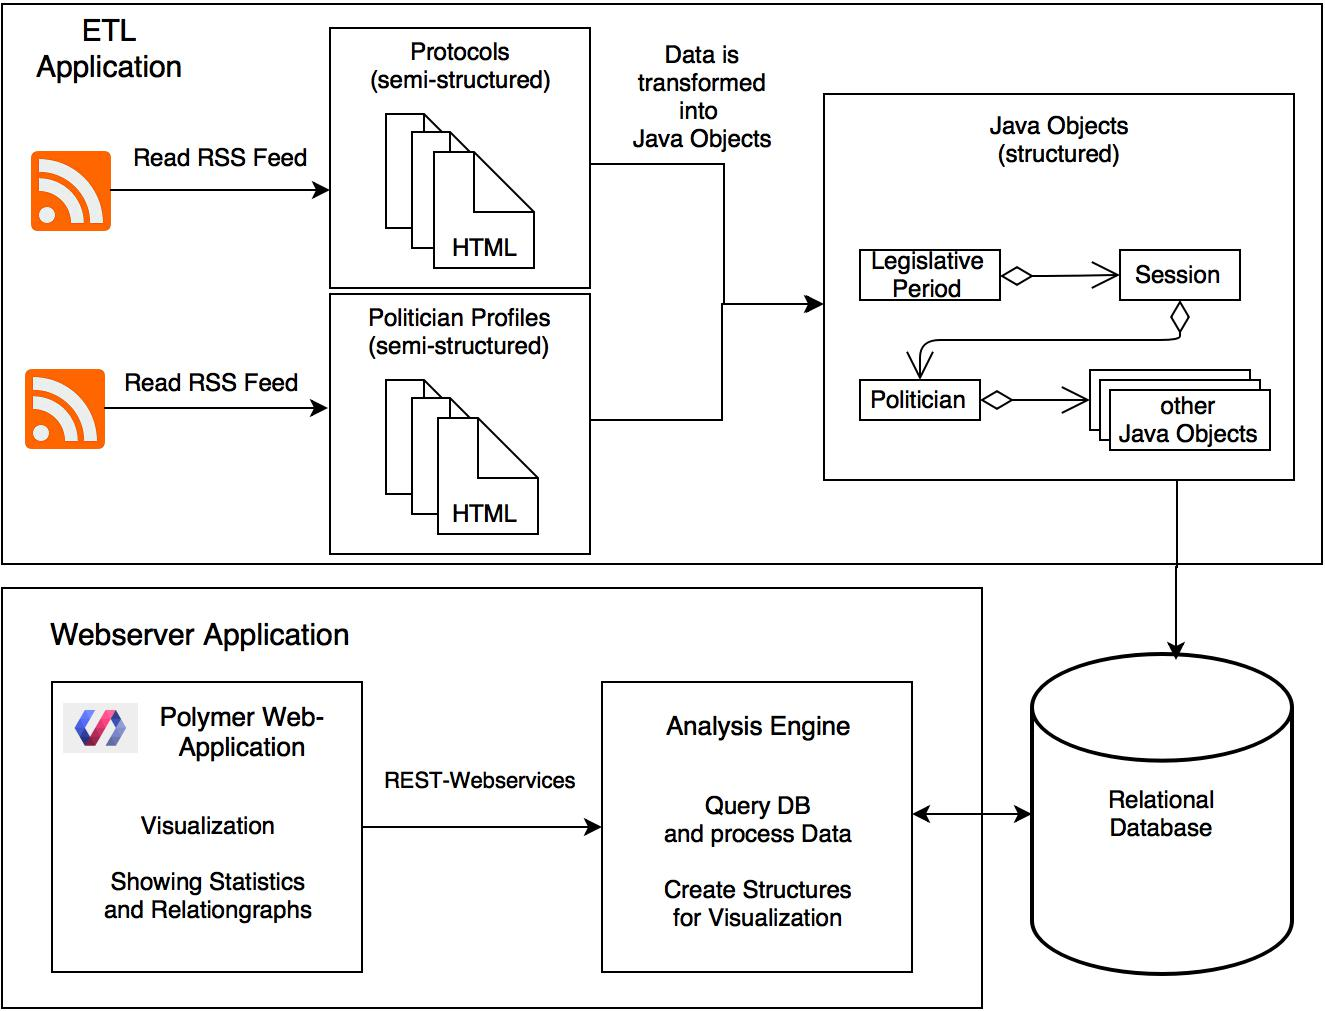
\includegraphics[width=\textwidth]{imgs/overall_architecture}
	\caption{General Architecture}
	\label{fig:general_architecture}
\end{figure}

\section{Data Extraction}
\label{sec:data_extraction_transforming}
The first step which has to be done in the ETL-Application is the extraction. The data which should be transformed has to be collected and stored. In our case the data is contained in the stenographic protocols of the national council and in politician profiles. Both the protocols and politician profiles are publicly available and can be found at the website of the Austrian parliament (See \url{https://www.parlament.gv.at/PAKT/STPROT/} and \url{https://www.parlament.gv.at/WWER/PARL/}). The protocols are available in PDF-format and since the $20^{th}$ legislative period also in HTML. As the transforming of the PDF-files would not result in sufficient quality, in this thesis only the HTML-files (the data since the $20^{th}$ legislative period) are being extracted and analyzed.

To collect the needed files automatically, RSS feeds are used. There are feeds available for both, stenographic protocols and politician profiles. The HTML-files which are linked in the feeds are being downloaded and stored on the file system before they are transformed.

\section{Transformation}
The next step is the transformation of the HTML-files into Java objects (transformation of semi-/unstructured data to structured data). To be able to extract the desired information out of the HTML-files, the structure of the stenographic protocols and politician profiles was investigated. Then undesired HTML-structures were removed, because they avoided a correct information extraction. For example, the page breaks and page headers in the full text protocols were removed. Then the tag structure of the HTML documents and regular expressions were used to find the required data.

\subsection{Transformation of the Politician Profiles}
%Figure \ref{fig:politician_profile_example} shows such a Profile. 
For each politician who is sitting in the national or federal council, there exists a politician profile. In the first part of the transformation, all politician profiles are being transformed into a list of politician Java objects. The name (and if provided previous names), the titles, the birth date, and the political mandates are being extracted from the HTML code. Mandates are some kind of political functions like the membership in the national or federal council or the period where the politician was a federal minister. They are important especially because they include the club memberships of the politician within a specific period of time. 
%To be able to extract these features out of the HTML code, the structure of the HTML file (e.g. the name of the politician is in the first <h1> tag of the page) and regular expressions are used. 
Figure \ref{fig:politicians_mandates_class_diagram} shows the class diagram of the resulting Java objects, extracted out of the profiles.

%\begin{figure}
%	\centering
%	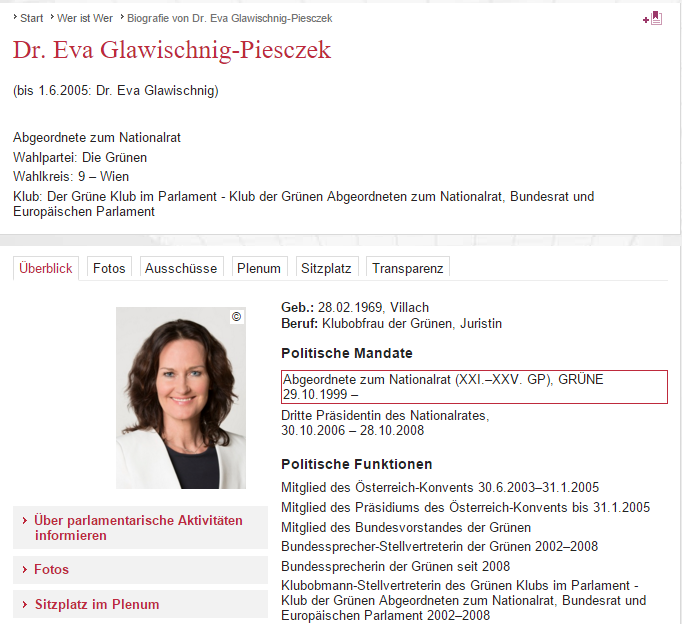
\includegraphics[width=341px]{imgs/politician_profile_example}
%	\caption{Example of a Politician Profile}
%	\label{fig:politician_profile_example}
%\end{figure}

\begin{figure}
	\centering
	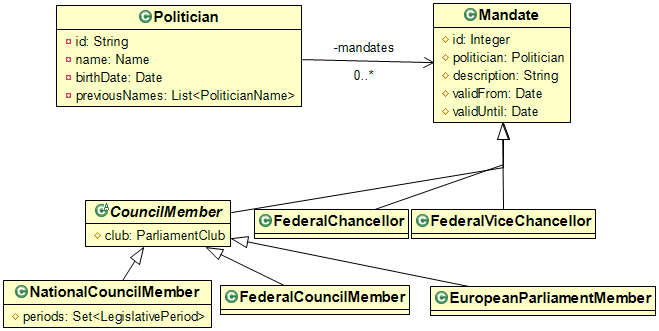
\includegraphics[width=\textwidth]{imgs/politicians_mandates_class_diagram}
	\caption{Class Diagram of the result of the Profile Transformation Step}
	\label{fig:politicians_mandates_class_diagram}
\end{figure}

\subsection{Transformation of the Protocols}
In the second part of the transformation, the protocols of the sessions of the national council are transformed. For each session, there exist two files: The full text protocol and the protocol summary. In the full text protocol there is every word which is being said in the session written down, whereas in the protocol summary, there is only important information like discussions and speeches summarized. Information that gets extracted out of the protocols includes sessions of legislative periods, chair men in the sessions, politician absences and presences, discussions and speeches of politicians. The list of politicians which was the result of the first transformation part is used to find the politicians in the protocols and to reference them in speeches. Figure \ref{fig:session_class_diagram} shows the class diagram of the resulting objects from the protocol transformation step.

\begin{figure}
	\centering
	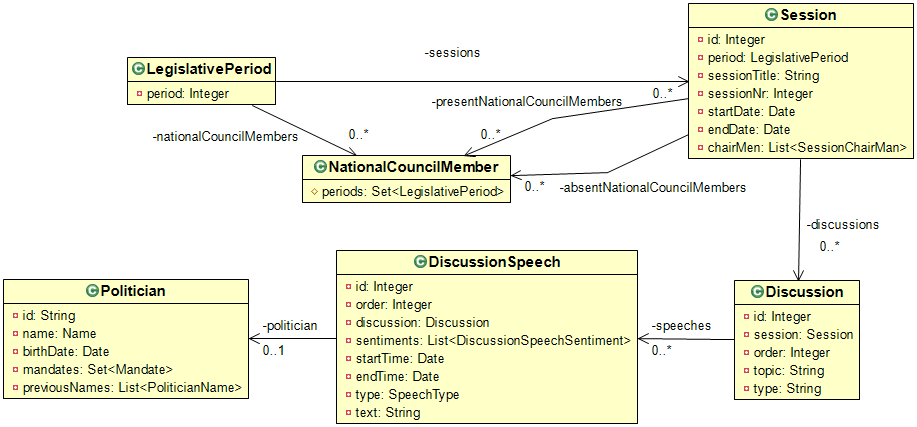
\includegraphics[width=\textwidth]{imgs/session_class_diagram}
	\caption{Class Diagram of the result of the Protocol Transformation Step}
	\label{fig:session_class_diagram}
\end{figure}


\section{Export into a Database}
\label{sec:export_db}
The export to a database is the loading part of the ETL application. The in the previous step created Java objects are being persisted into a relational database. To stay independent of specific databases the Java Persistence API and Hibernate are used. Using OR-mapping brings the advantages that no SQL-statements have to be written and changes on the tables/objects are easily made using Java annotations.

\section{Analysis}
\label{sec:analysis}

The first step of the analysis phase was to determine which analysis could be applied on the given data. The results can be classified into two categories: simple analysis and network analysis. The simple analysis takes just simple measures like how many speeches a politician held during a legislative period or how often was he absent. Table \ref{table:simple_analysis} shows all simple analysis measures taken. The network analysis will be discussed in section \ref{sec:network_analysis}.

\begin{table}
\begin{tabular}{| p{5cm} | p{8cm} |}
\hline
  Name & Description \\
\hline
\hline
  Overall Absence per Period & A percentage of the absence of all national council members in one legislative period. \\
\hline
Absence of a Politician per Period & A percentage of the absence of one national council member in one legislative period. \\
\hline
Absence of a Parliamentary club per Period & A percentage of the absence of all members of one parliamentary club in one legislative period. \\
\hline
Count of Speeches of politicians per Period & The count of speeches a politician held in the national council during one legislative period. \\
\hline

\end{tabular}

\caption{Simple Analysis Measures}
\label{table:simple_analysis}
\end{table}

\subsection{Network Analysis}
\label{sec:network_analysis}

\section{Visualization}
\label{sec:visualization}
